

% This document was generated by the publish-function
% from GNU Octave 4.2.1



\documentclass[10pt]{article}
\usepackage{listings}
\usepackage{mathtools}
\usepackage{amssymb}
\usepackage{graphicx}
\usepackage{hyperref}
\usepackage{xcolor}
\usepackage{titlesec}
\usepackage[utf8]{inputenc}
\usepackage[T1]{fontenc}
\usepackage{lmodern}


\lstset{
language=Octave,
numbers=none,
frame=single,
tabsize=2,
showstringspaces=false,
breaklines=true}


\titleformat*{\section}{\Huge\bfseries}
\titleformat*{\subsection}{\large\bfseries}
\renewcommand{\contentsname}{\Large\bfseries Contents}
\setlength{\parindent}{0pt}

\begin{document}

{\Huge\section*{test}}

\tableofcontents
\vspace*{4em}

\begin{lstlisting}
%%HomeWork 5
% 15307130224
%

%%Part one is shown within the *.jpeg file
\end{lstlisting}
\begin{lstlisting}[language={},xleftmargin=5pt,frame=none]

\end{lstlisting}


\phantomsection
\addcontentsline{toc}{section}{HouseHolder Function with test case}
\subsection*{HouseHolder Function with test case}

\begin{lstlisting}
%function [Q, A] = household(A)
%	[m, n] = size(A)
%
%	Q = eye(m)
%	for k = 1:n
%		x = A(k:m, k)
%
%		e = zeros(m-k+1, 1)
%		e(1,1) = 1

%		v_k = x + sign(x(1))*norm(x,2)*e
%		v_k = v_k/norm(v_k,2)
%
%		H = eye(m)
%		H(k:m,k:m) = eye(m-k+1) - 2*v_k*v_k'
%		A(k:m,k:n) = A(k:m,k:n) - 2*v_k*(v_k'*A(k:m,k:n));
%
%		Q = Q * H'
%	end

%end



error_of_my_self = zeros(10,1);
error_of_standard = zeros(10,1);
for i = 1:10
	a = rand(500);
	[Q_self,R_self] = household(a);
	[Q_standard, R_standard] = qr(a);

	error_of_my_self(i) = norm((Q_self*R_self-a), 'fro');
	error_of_standard(i) = norm((Q_standard*R_standard-a), 'fro');
end

mean_stand_error = mean(error_of_standard)
mean_self_error = mean(error_of_my_self)
\end{lstlisting}
\begin{lstlisting}[language={},xleftmargin=5pt,frame=none]
mean_stand_error =    2.6490e-13
mean_self_error =    1.0212e-12

\end{lstlisting}
\begin{lstlisting}
% We can use the least square mean error method to guess the paramter, to facilitate the
% process, we should use the QR decomposition and backward elimination.
%%Part3  Code
x_lines = linspace(0,1,30);
y_lines = zeros(30, 1);
A = zeros(30, 6);

for i = 1:30
	y_lines(i, 1) = cos(10*x_lines(i));
	for j = 1:6
		A(i,j) = x_lines(i)^(j-1);
	end
end

[Q, R] = household(A'*A);





lambdas = inv(R)*Q'*A'*y_lines

fit = zeros(30,1);
for i = 1:30
	for j = 1:6
		fit(i) = fit(i) + x_lines(i)^(j-1)*lambdas(j);
	end
end

plot(x_lines, fit, '-')
hold on
plot(x_lines, y_lines, '*')
\end{lstlisting}
\begin{lstlisting}[language={},xleftmargin=5pt,frame=none]
lambdas =
     0.98176
     4.72657
  -136.94707
   500.65066
  -637.23132
   267.17512

\end{lstlisting}
\begin{figure}[!ht]
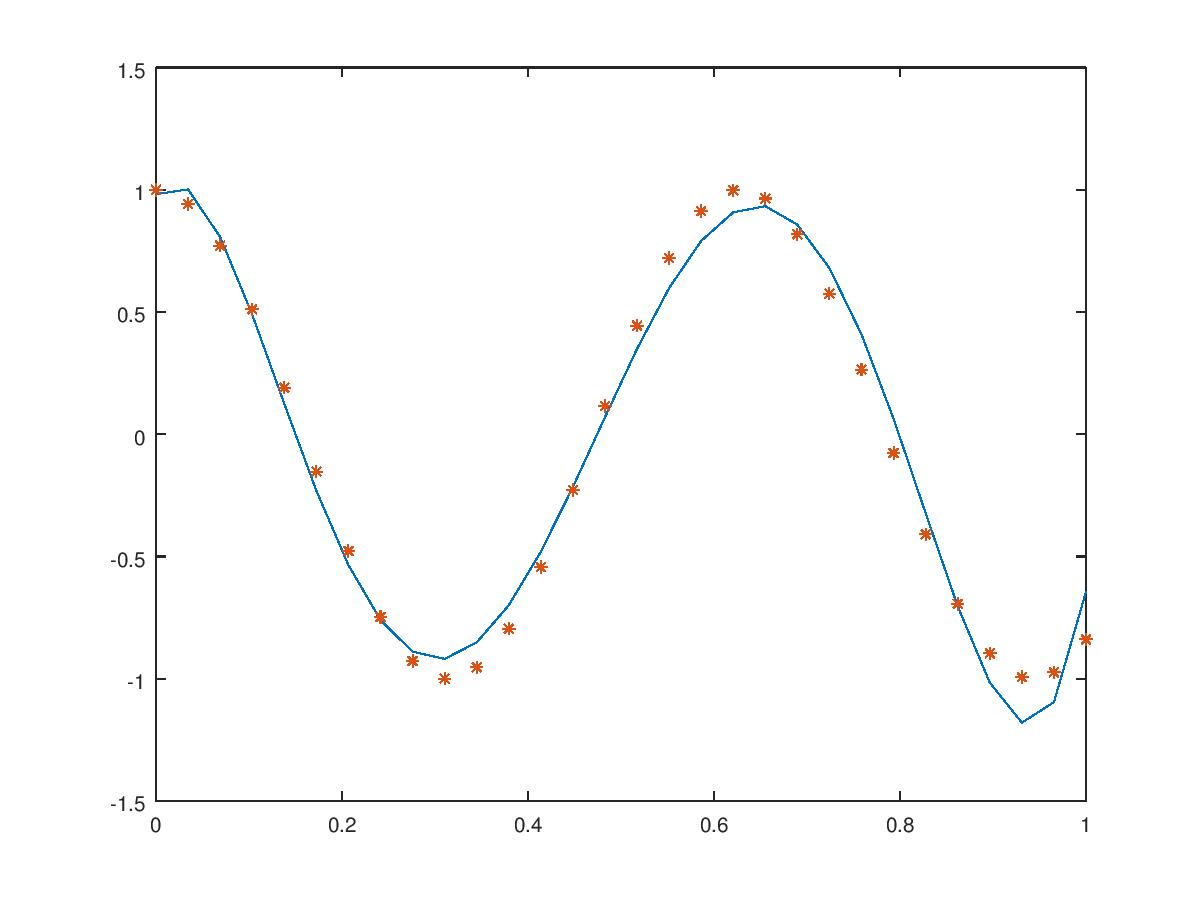
\includegraphics[width=\textwidth]{test-1.jpg}
\end{figure}


\end{document}
